\documentclass[]{article}
\usepackage{lmodern}
\usepackage{amssymb,amsmath}
\usepackage{ifxetex,ifluatex}
\usepackage{fixltx2e} % provides \textsubscript
\ifnum 0\ifxetex 1\fi\ifluatex 1\fi=0 % if pdftex
  \usepackage[T1]{fontenc}
  \usepackage[utf8]{inputenc}
\else % if luatex or xelatex
  \ifxetex
    \usepackage{mathspec}
  \else
    \usepackage{fontspec}
  \fi
  \defaultfontfeatures{Ligatures=TeX,Scale=MatchLowercase}
\fi
% use upquote if available, for straight quotes in verbatim environments
\IfFileExists{upquote.sty}{\usepackage{upquote}}{}
% use microtype if available
\IfFileExists{microtype.sty}{%
\usepackage{microtype}
\UseMicrotypeSet[protrusion]{basicmath} % disable protrusion for tt fonts
}{}
\usepackage[margin=1in]{geometry}
\usepackage{hyperref}
\hypersetup{unicode=true,
            pdftitle={EVBB Analysis},
            pdfauthor={Rafferty Parker (University of Otago)},
            pdfborder={0 0 0},
            breaklinks=true}
\urlstyle{same}  % don't use monospace font for urls
\usepackage{color}
\usepackage{fancyvrb}
\newcommand{\VerbBar}{|}
\newcommand{\VERB}{\Verb[commandchars=\\\{\}]}
\DefineVerbatimEnvironment{Highlighting}{Verbatim}{commandchars=\\\{\}}
% Add ',fontsize=\small' for more characters per line
\usepackage{framed}
\definecolor{shadecolor}{RGB}{248,248,248}
\newenvironment{Shaded}{\begin{snugshade}}{\end{snugshade}}
\newcommand{\KeywordTok}[1]{\textcolor[rgb]{0.13,0.29,0.53}{\textbf{#1}}}
\newcommand{\DataTypeTok}[1]{\textcolor[rgb]{0.13,0.29,0.53}{#1}}
\newcommand{\DecValTok}[1]{\textcolor[rgb]{0.00,0.00,0.81}{#1}}
\newcommand{\BaseNTok}[1]{\textcolor[rgb]{0.00,0.00,0.81}{#1}}
\newcommand{\FloatTok}[1]{\textcolor[rgb]{0.00,0.00,0.81}{#1}}
\newcommand{\ConstantTok}[1]{\textcolor[rgb]{0.00,0.00,0.00}{#1}}
\newcommand{\CharTok}[1]{\textcolor[rgb]{0.31,0.60,0.02}{#1}}
\newcommand{\SpecialCharTok}[1]{\textcolor[rgb]{0.00,0.00,0.00}{#1}}
\newcommand{\StringTok}[1]{\textcolor[rgb]{0.31,0.60,0.02}{#1}}
\newcommand{\VerbatimStringTok}[1]{\textcolor[rgb]{0.31,0.60,0.02}{#1}}
\newcommand{\SpecialStringTok}[1]{\textcolor[rgb]{0.31,0.60,0.02}{#1}}
\newcommand{\ImportTok}[1]{#1}
\newcommand{\CommentTok}[1]{\textcolor[rgb]{0.56,0.35,0.01}{\textit{#1}}}
\newcommand{\DocumentationTok}[1]{\textcolor[rgb]{0.56,0.35,0.01}{\textbf{\textit{#1}}}}
\newcommand{\AnnotationTok}[1]{\textcolor[rgb]{0.56,0.35,0.01}{\textbf{\textit{#1}}}}
\newcommand{\CommentVarTok}[1]{\textcolor[rgb]{0.56,0.35,0.01}{\textbf{\textit{#1}}}}
\newcommand{\OtherTok}[1]{\textcolor[rgb]{0.56,0.35,0.01}{#1}}
\newcommand{\FunctionTok}[1]{\textcolor[rgb]{0.00,0.00,0.00}{#1}}
\newcommand{\VariableTok}[1]{\textcolor[rgb]{0.00,0.00,0.00}{#1}}
\newcommand{\ControlFlowTok}[1]{\textcolor[rgb]{0.13,0.29,0.53}{\textbf{#1}}}
\newcommand{\OperatorTok}[1]{\textcolor[rgb]{0.81,0.36,0.00}{\textbf{#1}}}
\newcommand{\BuiltInTok}[1]{#1}
\newcommand{\ExtensionTok}[1]{#1}
\newcommand{\PreprocessorTok}[1]{\textcolor[rgb]{0.56,0.35,0.01}{\textit{#1}}}
\newcommand{\AttributeTok}[1]{\textcolor[rgb]{0.77,0.63,0.00}{#1}}
\newcommand{\RegionMarkerTok}[1]{#1}
\newcommand{\InformationTok}[1]{\textcolor[rgb]{0.56,0.35,0.01}{\textbf{\textit{#1}}}}
\newcommand{\WarningTok}[1]{\textcolor[rgb]{0.56,0.35,0.01}{\textbf{\textit{#1}}}}
\newcommand{\AlertTok}[1]{\textcolor[rgb]{0.94,0.16,0.16}{#1}}
\newcommand{\ErrorTok}[1]{\textcolor[rgb]{0.64,0.00,0.00}{\textbf{#1}}}
\newcommand{\NormalTok}[1]{#1}
\usepackage{longtable,booktabs}
\usepackage{graphicx,grffile}
\makeatletter
\def\maxwidth{\ifdim\Gin@nat@width>\linewidth\linewidth\else\Gin@nat@width\fi}
\def\maxheight{\ifdim\Gin@nat@height>\textheight\textheight\else\Gin@nat@height\fi}
\makeatother
% Scale images if necessary, so that they will not overflow the page
% margins by default, and it is still possible to overwrite the defaults
% using explicit options in \includegraphics[width, height, ...]{}
\setkeys{Gin}{width=\maxwidth,height=\maxheight,keepaspectratio}
\IfFileExists{parskip.sty}{%
\usepackage{parskip}
}{% else
\setlength{\parindent}{0pt}
\setlength{\parskip}{6pt plus 2pt minus 1pt}
}
\setlength{\emergencystretch}{3em}  % prevent overfull lines
\providecommand{\tightlist}{%
  \setlength{\itemsep}{0pt}\setlength{\parskip}{0pt}}
\setcounter{secnumdepth}{5}
% Redefines (sub)paragraphs to behave more like sections
\ifx\paragraph\undefined\else
\let\oldparagraph\paragraph
\renewcommand{\paragraph}[1]{\oldparagraph{#1}\mbox{}}
\fi
\ifx\subparagraph\undefined\else
\let\oldsubparagraph\subparagraph
\renewcommand{\subparagraph}[1]{\oldsubparagraph{#1}\mbox{}}
\fi

%%% Use protect on footnotes to avoid problems with footnotes in titles
\let\rmarkdownfootnote\footnote%
\def\footnote{\protect\rmarkdownfootnote}

%%% Change title format to be more compact
\usepackage{titling}

% Create subtitle command for use in maketitle
\newcommand{\subtitle}[1]{
  \posttitle{
    \begin{center}\large#1\end{center}
    }
}

\setlength{\droptitle}{-2em}

  \title{EVBB Analysis}
    \pretitle{\vspace{\droptitle}\centering\huge}
  \posttitle{\par}
  \subtitle{subtitle goes here}
  \author{Rafferty Parker (University of Otago)}
    \preauthor{\centering\large\emph}
  \postauthor{\par}
      \predate{\centering\large\emph}
  \postdate{\par}
    \date{Last run at: 2018-12-14 13:47:45}


\begin{document}
\maketitle

{
\setcounter{tocdepth}{2}
\tableofcontents
}
\section{Introduction}\label{introduction}

New Zealand's total electricity demand varies throughout the day, with
two distinct ``peaks''; one in the morning, and one in the evening.
Providing the electicity to meet these demand peaks is a costly and
inefficient process. If poorly managed, the increase in electric
vehicles may increase these daily peaks significantly
{[}@stephenson\_smart\_2017{]}.

When/where is the greatest amount of charging occurring? What is the
power demand per vehicle/household/place of charging? What might this
look like if 50\% of households had an EV? What about if it matched
current ICE ownership (eventually)?

Develop tools for analyzing the data so that data can be fed in and
plots automatically constructed

\section{Brief literature review}\label{brief-literature-review}

While some work has been done in quantifying the extent of this
problem{[}@concept\_2018{]}, these have been conducted based on
estimations of charging patterns based on current driver behaviour.

The New Zealand government has set a target of increasing the number of
EVs in New Zealand to 64,000 by 2021.

In contrast, this report uses actual data collected from EV

What do we already know (or suspect) about when they will be charged.
Include:

\begin{itemize}
\tightlist
\item
  academic literature
\item
  consultant reports
\item
  etc
\end{itemize}

This is an example of a bibtex reference to a paper:
{[}@stephenson\_smart\_2017{]}

This is an example of a reference to an R package: {[}@dplyr{]}

\section{Research questions}\label{research-questions}

Break down the main questions \& refer back to the literature

\section{Methods}\label{methods}

\subsection{Data}\label{data}

Describe it:

The data used has been provided by ``Flip the Fleet'', a community
organisation that hopes to increase uptake of electric vehicles in New
Zealand. Flip the Fleet have been collecting data on electric vehicle
usage patterns, collected using Exact IOT Limited's ``Black Box'', a
small electronic device that connects to the internal computer and sends
detailed data about the EV's ``battery health, consumption, speed,
etc.''.

The data has been anonymised through the hashing of license plate
numbers and dates.

Charging data has been broadly seperated into two seperate catagories,
``slow'' and ``fast''. Slow charging is when the charger is reading less
than 7kW - this is considered the upper limit of what can be obtained
from a standard home charging scenario without an expensive wiring
upgrade. Fast charging is all charging above 7kw, and would likely occur
at designated and purpose-built fast charging stations.

Grid peaks are more pronounced during weekdays. Because of this, the
data was also catagorised according to whether it was a weekday or not.
This allows analysis to occur of differing charging patterns between
weekdays and weekends, allowing for further accuracy in determining the
effects of grid peaks.

\begin{itemize}
\tightlist
\item
  where did you get it?
\item
  how many vehicles, where are they and what kinds?
\item
  anything we need to know about the data?
\item
  what did you have to do to it (cleaning etc)
\item
  descriptive analysis, e.g.:
\item
  Plot all charging with fast and slow charges differentiated
\item
  Plot fast charges with weekend and weekday differentiated
\item
  Histograms of power (kW)
\end{itemize}

Load the data - note the feedback readr gives you on the assumed format
of the columns. You might \emph{not} want to remove the original
dateTime :-)

\begin{Shaded}
\begin{Highlighting}[]
\NormalTok{df <-}\StringTok{ }\NormalTok{readr}\OperatorTok{::}\KeywordTok{read_csv}\NormalTok{(iFile)}
\end{Highlighting}
\end{Shaded}

\begin{verbatim}
## Parsed with column specification:
## cols(
##   id = col_character(),
##   dayid = col_character(),
##   month = col_character(),
##   day_of_week = col_character(),
##   time = col_time(format = ""),
##   fractime = col_double(),
##   charge_power_kw = col_double(),
##   location = col_character()
## )
\end{verbatim}

This is a cross-references to Table \ref{tab:tab1}.

\begin{Shaded}
\begin{Highlighting}[]
\NormalTok{t <-}\StringTok{ }\KeywordTok{summary}\NormalTok{(df)}

\NormalTok{knitr}\OperatorTok{::}\KeywordTok{kable}\NormalTok{(t, }\DataTypeTok{caption =} \StringTok{"Data summary"}\NormalTok{) }\CommentTok{# <- makes a pretty table}
\end{Highlighting}
\end{Shaded}

\begin{table}

\caption{\label{tab:tab1}Data summary}
\centering
\begin{tabular}[t]{l|l|l|l|l|l|l|l|l}
\hline
  &      id &    dayid &    month & day\_of\_week &     time &    fractime & charge\_power\_kw &   location\\
\hline
 & Length:40993 & Length:40993 & Length:40993 & Length:40993 & Length:40993 & Min.   : 0.000 & Min.   : 0.000 & Length:40993\\
\hline
 & Class :character & Class :character & Class :character & Class :character & Class1:hms & 1st Qu.: 5.194 & 1st Qu.: 2.213 & Class :character\\
\hline
 & Mode  :character & Mode  :character & Mode  :character & Mode  :character & Class2:difftime & Median :12.258 & Median : 2.844 & Mode  :character\\
\hline
 & NA & NA & NA & NA & Mode  :numeric & Mean   :11.884 & Mean   : 2.729 & NA\\
\hline
 & NA & NA & NA & NA & NA & 3rd Qu.:18.318 & 3rd Qu.: 3.004 & NA\\
\hline
 & NA & NA & NA & NA & NA & Max.   :24.000 & Max.   :49.354 & NA\\
\hline
\end{tabular}
\end{table}

\begin{Shaded}
\begin{Highlighting}[]
\NormalTok{df}\OperatorTok{$}\NormalTok{day_of_week <-}\StringTok{ }\KeywordTok{factor}\NormalTok{(df}\OperatorTok{$}\NormalTok{day_of_week, }\DataTypeTok{ordered =} \OtherTok{TRUE}\NormalTok{,}
                                     \DataTypeTok{levels =} \KeywordTok{c}\NormalTok{(}\StringTok{"Monday"}\NormalTok{, }\StringTok{"Tuesday"}\NormalTok{, }\StringTok{"Wednesday"}\NormalTok{,}\StringTok{"Thursday"}\NormalTok{,}
                                                \StringTok{"Friday"}\NormalTok{, }\StringTok{"Saturday"}\NormalTok{, }\StringTok{"Sunday"}\NormalTok{)) }
\NormalTok{df}\OperatorTok{$}\NormalTok{month <-}\StringTok{ }\KeywordTok{factor}\NormalTok{(df}\OperatorTok{$}\NormalTok{month, }\DataTypeTok{ordered =} \OtherTok{TRUE}\NormalTok{, }\DataTypeTok{levels =} \KeywordTok{c}\NormalTok{(}\StringTok{"Jan"}\NormalTok{, }\StringTok{"Feb"}\NormalTok{, }\StringTok{"Mar"}\NormalTok{, }\StringTok{"Apr"}\NormalTok{, }\StringTok{"May"}\NormalTok{,}
                                                        \StringTok{"Jun"}\NormalTok{, }\StringTok{"Jul"}\NormalTok{, }\StringTok{"Aug"}\NormalTok{, }\StringTok{"Sep"}\NormalTok{, }\StringTok{"Oct"}\NormalTok{,}
                                                        \StringTok{"Nov"}\NormalTok{, }\StringTok{"Dec"}\NormalTok{))}

\NormalTok{weekdays1 <-}\StringTok{ }\KeywordTok{c}\NormalTok{(}\StringTok{"Monday"}\NormalTok{, }\StringTok{"Tuesday"}\NormalTok{, }\StringTok{"Wednesday"}\NormalTok{, }\StringTok{"Thursday"}\NormalTok{, }\StringTok{"Friday"}\NormalTok{)}
\NormalTok{df}\OperatorTok{$}\NormalTok{weekday <-}\StringTok{ }\KeywordTok{factor}\NormalTok{((df}\OperatorTok{$}\NormalTok{day_of_week }\OperatorTok\StringTok{ }\NormalTok{weekdays1), }
                   \DataTypeTok{levels =} \KeywordTok{c}\NormalTok{(}\OtherTok{FALSE}\NormalTok{, }\OtherTok{TRUE}\NormalTok{), }\DataTypeTok{labels =} \KeywordTok{c}\NormalTok{(}\StringTok{'Weekend'}\NormalTok{, }\StringTok{'Weekday'}\NormalTok{)) }

\NormalTok{df}\OperatorTok{$}\NormalTok{charging_rate <-}\StringTok{ }\KeywordTok{factor}\NormalTok{((df}\OperatorTok{$}\NormalTok{charge_power_kw }\OperatorTok{>=}\StringTok{ }\DecValTok{7}\NormalTok{),}
                    \DataTypeTok{levels =} \KeywordTok{c}\NormalTok{(}\OtherTok{TRUE}\NormalTok{, }\OtherTok{FALSE}\NormalTok{), }\DataTypeTok{labels =} \KeywordTok{c}\NormalTok{(}\StringTok{'Fast'}\NormalTok{, }\StringTok{'Slow'}\NormalTok{),}
                    \DataTypeTok{ordered =} \OtherTok{TRUE}\NormalTok{)}
\end{Highlighting}
\end{Shaded}

\begin{Shaded}
\begin{Highlighting}[]
\NormalTok{df}\OperatorTok{$}\NormalTok{halfHour <-}\StringTok{ }\KeywordTok{format}\NormalTok{(}\KeywordTok{as.POSIXct}\NormalTok{(hms}\OperatorTok{::}\KeywordTok{trunc_hms}\NormalTok{(df}\OperatorTok{$}\NormalTok{time, }\DecValTok{30}\OperatorTok{*}\DecValTok{60}\NormalTok{)), }\StringTok{"%H:%M"}\NormalTok{) }\CommentTok{# <- code to half hours, removing seconds}
\end{Highlighting}
\end{Shaded}

\begin{Shaded}
\begin{Highlighting}[]
\NormalTok{df}\OperatorTok{$}\NormalTok{id <-}\StringTok{ }\KeywordTok{factor}\NormalTok{(df}\OperatorTok{$}\NormalTok{id, }\DataTypeTok{ordered =} \OtherTok{TRUE}\NormalTok{)}
\NormalTok{levSeq <-}\StringTok{ }\KeywordTok{seq}\NormalTok{(}\DecValTok{1}\OperatorTok{:}\KeywordTok{length}\NormalTok{(}\KeywordTok{levels}\NormalTok{(df}\OperatorTok{$}\NormalTok{id)))}
\NormalTok{levSeqChar <-}\StringTok{ }\KeywordTok{as.character}\NormalTok{(levSeq)}

\NormalTok{df}\OperatorTok{$}\NormalTok{id <-}\StringTok{ }\KeywordTok{factor}\NormalTok{(df}\OperatorTok{$}\NormalTok{id,}
  \DataTypeTok{labels =}\NormalTok{ levSeqChar)}

\NormalTok{df}\OperatorTok{$}\NormalTok{id <-}\StringTok{ }\KeywordTok{as.character}\NormalTok{(df}\OperatorTok{$}\NormalTok{id)}

\NormalTok{df}\OperatorTok{$}\NormalTok{id <-}\StringTok{ }\KeywordTok{paste}\NormalTok{(}\StringTok{"Vehicle"}\NormalTok{, df}\OperatorTok{$}\NormalTok{id, }\DataTypeTok{sep =} \StringTok{" "}\NormalTok{)}


\CommentTok{# It *might* be useful to do a similar thing with dayid, however it appears there is a seperate dayid per car per day (not same for different cars on same day)}
\CommentTok{# This would be unnecessary if I get a proper datetime stamp}
\end{Highlighting}
\end{Shaded}

Figure \ref{fig:plot1} implies that most charging is ``slow''.

\begin{Shaded}
\begin{Highlighting}[]
\NormalTok{p <-}\StringTok{ }\NormalTok{ggplot2}\OperatorTok{::}\KeywordTok{ggplot}\NormalTok{(df, }\KeywordTok{aes}\NormalTok{(}\DataTypeTok{x =}\NormalTok{ charge_power_kw)) }\OperatorTok{+}
\StringTok{  }\KeywordTok{guides}\NormalTok{(}\DataTypeTok{colour =} \KeywordTok{guide_legend}\NormalTok{(}\DataTypeTok{title =} \StringTok{"Vehicle:"}\NormalTok{)) }\OperatorTok{+}
\StringTok{  }\KeywordTok{theme}\NormalTok{(}\DataTypeTok{legend.position=}\StringTok{"bottom"}\NormalTok{) }\OperatorTok{+}
\StringTok{  }\KeywordTok{scale_colour_manual}\NormalTok{(}\DataTypeTok{values=}\NormalTok{cbPalette) }\OperatorTok{+}\StringTok{ }\CommentTok{# use colour-blind friendly palette}
\StringTok{  }\KeywordTok{geom_density}\NormalTok{() }\CommentTok{# <- make the plot in an object first}

\NormalTok{p }\OperatorTok{+}\StringTok{ }\KeywordTok{labs}\NormalTok{(}\DataTypeTok{x =} \StringTok{"Power (kW)"}\NormalTok{) }\OperatorTok{+}\StringTok{ }\KeywordTok{facet_grid}\NormalTok{(id }\OperatorTok{~}\StringTok{ }\NormalTok{.) }\OperatorTok{+}
\StringTok{    }\KeywordTok{annotate}\NormalTok{(}\StringTok{"rect"}\NormalTok{, }\DataTypeTok{xmin =} \DecValTok{0}\NormalTok{, }\DataTypeTok{xmax =} \DecValTok{7}\NormalTok{, }\DataTypeTok{ymin =} \DecValTok{0}\NormalTok{, }\DataTypeTok{ymax =} \FloatTok{1.5}\NormalTok{,}
           \DataTypeTok{alpha =} \FloatTok{.1}\NormalTok{, }\DataTypeTok{fill=}\StringTok{"yellow"}\NormalTok{) }\OperatorTok{+}
\StringTok{  }\KeywordTok{annotate}\NormalTok{(}\StringTok{"rect"}\NormalTok{, }\DataTypeTok{xmin =} \DecValTok{7}\NormalTok{, }\DataTypeTok{xmax =} \DecValTok{50}\NormalTok{, }\DataTypeTok{ymin =} \DecValTok{0}\NormalTok{, }\DataTypeTok{ymax =} \FloatTok{1.5}\NormalTok{,}
           \DataTypeTok{alpha =} \FloatTok{.1}\NormalTok{, }\DataTypeTok{fill=}\StringTok{"blue"}\NormalTok{) }\OperatorTok{+}
\StringTok{  }\KeywordTok{annotate}\NormalTok{(}\StringTok{"text"}\NormalTok{,}\DataTypeTok{label=}\StringTok{"Slow"}\NormalTok{, }\DataTypeTok{x=}\FloatTok{3.5}\NormalTok{, }\DataTypeTok{y=}\FloatTok{1.25}\NormalTok{, }\DataTypeTok{angle=}\DecValTok{0}\NormalTok{) }\OperatorTok{+}
\StringTok{  }\KeywordTok{annotate}\NormalTok{(}\StringTok{"text"}\NormalTok{,}\DataTypeTok{label=}\StringTok{"Fast"}\NormalTok{, }\DataTypeTok{x=}\NormalTok{(}\DecValTok{50-7}\NormalTok{)}\OperatorTok{/}\DecValTok{2} \OperatorTok{+}\StringTok{ }\DecValTok{7}\NormalTok{, }\DataTypeTok{y=}\FloatTok{1.25}\NormalTok{, }\DataTypeTok{angle=}\DecValTok{0}\NormalTok{)}
\end{Highlighting}
\end{Shaded}

\begin{figure}
\centering
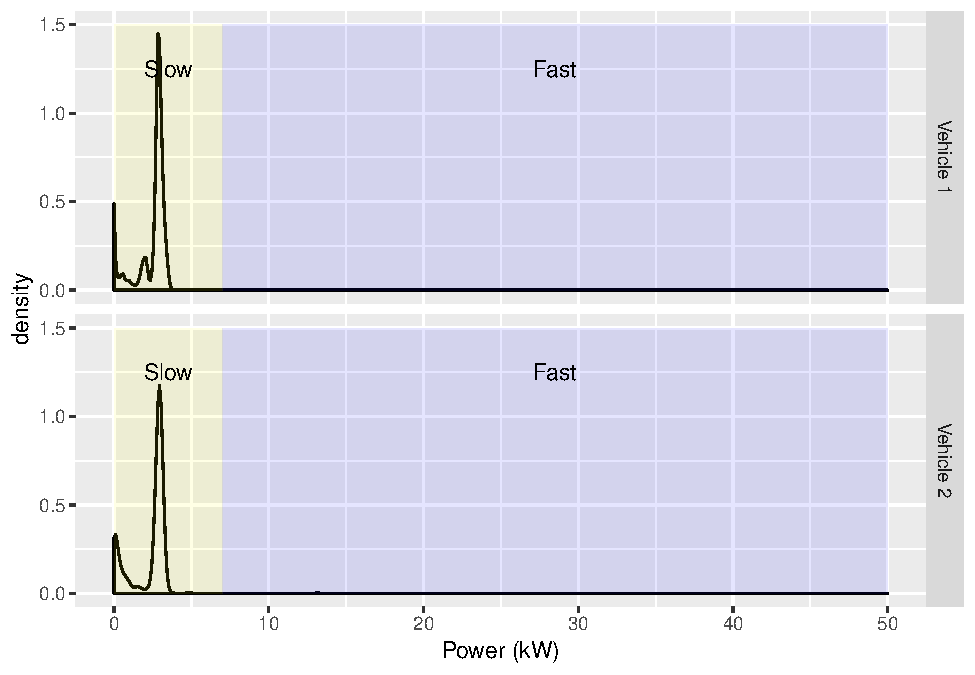
\includegraphics{EVBB_Report_files/figure-latex/plot1-1.pdf}
\caption{\label{fig:plot1}Density plot of charging power by car}
\end{figure}

\begin{Shaded}
\begin{Highlighting}[]
\CommentTok{# Not sure the annotations are really necessary but will leave them for now}
\CommentTok{# Also probably don't need two different colours for each car}
\end{Highlighting}
\end{Shaded}

\subsection{Analysis}\label{analysis}

Analysis was conducted using R (R version 3.4.4 (2018-03-15)) and the
following packages:

\begin{itemize}
\tightlist
\item
  ggplot2 {[}@ggplot2{]}
\item
  dplyr {[}@dplyr{]}
\end{itemize}

Reports were developed using knitr {[}@knitr{]} within bookdown
{[}@bookdown{]}.

\section{Charging Analysis}\label{charging-analysis}

\subsection{Research question 1}\label{research-question-1}

When does charging happen?

This is a cross-reference to Figure \ref{fig:plot2}. Time is coded to
half hours.

\begin{Shaded}
\begin{Highlighting}[]
\NormalTok{p <-}\StringTok{ }\NormalTok{ggplot2}\OperatorTok{::}\KeywordTok{ggplot}\NormalTok{(df, }\KeywordTok{aes}\NormalTok{(}\DataTypeTok{x =}\NormalTok{ halfHour, }\DataTypeTok{group =}\NormalTok{ halfHour, }\DataTypeTok{y =}\NormalTok{ charge_power_kw)) }\OperatorTok{+}
\StringTok{  }\KeywordTok{guides}\NormalTok{(}\DataTypeTok{colour =} \KeywordTok{guide_legend}\NormalTok{(}\DataTypeTok{title =} \StringTok{"Vehicle:"}\NormalTok{)) }\OperatorTok{+}
\StringTok{  }\KeywordTok{theme}\NormalTok{(}\DataTypeTok{legend.position=}\StringTok{"bottom"}\NormalTok{) }\OperatorTok{+}
\StringTok{  }\KeywordTok{scale_colour_manual}\NormalTok{(}\DataTypeTok{values=}\NormalTok{cbPalette) }\OperatorTok{+}\StringTok{ }\CommentTok{# use colour-blind friendly palette}
\StringTok{  }\KeywordTok{geom_boxplot}\NormalTok{() }\CommentTok{# <- make the plot in an object first}

\NormalTok{p }\OperatorTok{+}\StringTok{ }\KeywordTok{labs}\NormalTok{(}\DataTypeTok{x =} \StringTok{"Time of Day"}\NormalTok{, }\DataTypeTok{y =} \StringTok{"Power (kW)"}\NormalTok{) }\OperatorTok{+}\StringTok{ }\KeywordTok{facet_grid}\NormalTok{(day_of_week }\OperatorTok{~}\StringTok{ }\NormalTok{id)}
\end{Highlighting}
\end{Shaded}

\begin{figure}
\centering
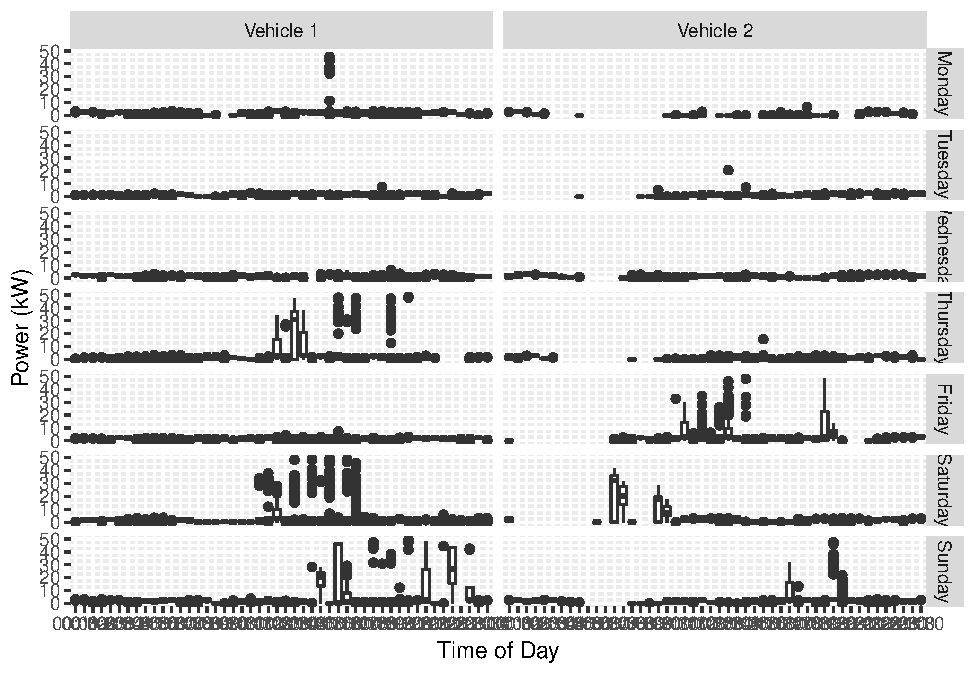
\includegraphics{EVBB_Report_files/figure-latex/plot2-1.pdf}
\caption{\label{fig:plot2}Boxplot of charging timing by car}
\end{figure}

\begin{Shaded}
\begin{Highlighting}[]
\NormalTok{p <-}\StringTok{ }\NormalTok{ggplot2}\OperatorTok{::}\KeywordTok{ggplot}\NormalTok{(df, }\KeywordTok{aes}\NormalTok{(}\DataTypeTok{x =}\NormalTok{ halfHour, }\DataTypeTok{group =}\NormalTok{ halfHour, }\DataTypeTok{y =}\NormalTok{ charge_power_kw)) }\OperatorTok{+}
\StringTok{  }\KeywordTok{guides}\NormalTok{(}\DataTypeTok{colour =} \KeywordTok{guide_legend}\NormalTok{(}\DataTypeTok{title =} \StringTok{"Vehicle:"}\NormalTok{)) }\OperatorTok{+}
\StringTok{  }\KeywordTok{theme}\NormalTok{(}\DataTypeTok{legend.position=}\StringTok{"bottom"}\NormalTok{) }\OperatorTok{+}
\StringTok{  }\KeywordTok{scale_colour_manual}\NormalTok{(}\DataTypeTok{values=}\NormalTok{cbPalette) }\OperatorTok{+}\StringTok{ }\CommentTok{# use colour-blind friendly palette}
\StringTok{  }\KeywordTok{geom_boxplot}\NormalTok{() }\OperatorTok{+}
\StringTok{  }\KeywordTok{stat_summary}\NormalTok{(}\KeywordTok{aes}\NormalTok{(}\DataTypeTok{group =}\NormalTok{ weekday), }\DataTypeTok{fun.y=}\NormalTok{mean, }\DataTypeTok{geom=}\StringTok{"line"}\NormalTok{, }\DataTypeTok{colour =} \StringTok{"red"}\NormalTok{) }\OperatorTok{+}
\StringTok{  }\KeywordTok{coord_cartesian}\NormalTok{(}\DataTypeTok{xlim =} \KeywordTok{c}\NormalTok{(}\DecValTok{0}\NormalTok{,}\DecValTok{24}\NormalTok{),}\DataTypeTok{ylim=}\KeywordTok{c}\NormalTok{(}\DecValTok{0}\NormalTok{,}\DecValTok{15}\NormalTok{))}

\NormalTok{p }\OperatorTok{+}\StringTok{ }\KeywordTok{labs}\NormalTok{(}\DataTypeTok{x =} \StringTok{"Time of Day"}\NormalTok{, }\DataTypeTok{y =} \StringTok{"Power (kW)"}\NormalTok{) }\OperatorTok{+}\StringTok{ }\KeywordTok{facet_grid}\NormalTok{(}\OperatorTok{~}\NormalTok{weekday) }
\end{Highlighting}
\end{Shaded}

\begin{figure}
\centering
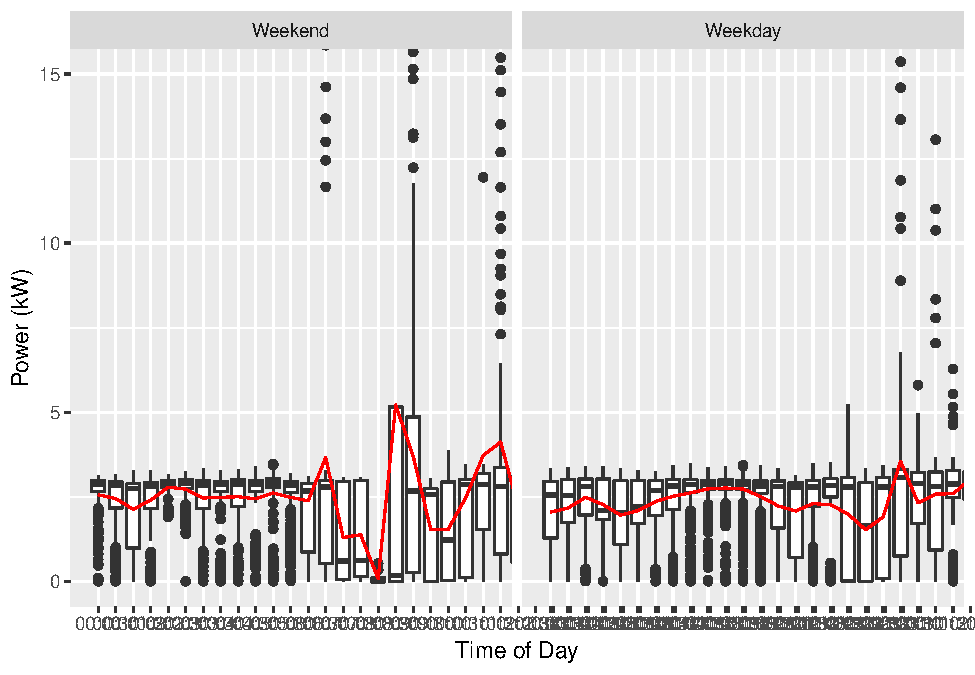
\includegraphics{EVBB_Report_files/figure-latex/plot3-1.pdf}
\caption{\label{fig:plot3}Weekend and weekday charging patterns}
\end{figure}

\subsection{Research question 2}\label{research-question-2}

How might this affect the NZ electricity grid?

\section{Conclusions}\label{conclusions}

\section{References}\label{references}


\end{document}
